\documentclass[12pt]{scrartcl}
\usepackage{graphicx}
\usepackage{float}
\usepackage[figurename=Figure]{caption}
\usepackage{verbatim} % For comments and other
\usepackage{amsmath}  % For math
\usepackage{amssymb}  % For more math
\usepackage{fullpage}
\usepackage{paralist} % paragraph spacing
\usepackage{listings} % For source code
\usepackage{subfig}

\usepackage{enumitem} % useful for itemization
\usepackage{siunitx}  % standardization of si units

\usepackage{tikz,bm} % Useful for drawing plots
\usepackage{tikz-3dplot}

\usepackage{setspace}
\usepackage{geometry}

\geometry{
left=20mm,
top=10mm,
bottom=10mm,
}

\Large


\begin{document}

\onehalfspacing
\newcommand{\current}{June 2023}
\begin{center}
\hrule
\vspace{.4cm}
{\textbf { \large COL334 Computer Networks SEM II 2023-24}}
\end{center}
{
    \begin{center}
        Vatsal Jingar (2020CS50449)\\ Stitiprajna Sahoo (2020CS10394)\\ Tanish Gupta (2020CS10397)\\
        \textbf{Date:} 8 September 2023 \\
        \textbf{Assignment 2: Mimicking distributed file transfer}
    
    \end{center}
{ 
    \hrule
}
}
\section{Implementation Cpp (g++ 10.4)}
\begin{enumerate}
    \item \textbf{clientburst.cpp}\\
    This file contains the code logic for receving packets continuously from the server.
    \item \textbf{clientrecv.cpp}\\
    Client will receive the packets continuously from its peer cleint.
    \item \textbf{cleintbroadcast.cpp}\\
    Client will broadcast the packets to its peer clients continuously.
    \item \textbf{controller.cpp}\\
    Every client will keep count of how much lines it has received. When it is L = 1000, it will communicate it with the main thread.
    \item \textbf{driver.cpp}\\
    Every client can run this file with their respective ip written in constants.h.
    \item \textbf{constants.h}\\
    All the constants like Number of cleints, port number, ip address of clients are written here.
\end{enumerate}





\subsection{Code Structure}
\begin{center}
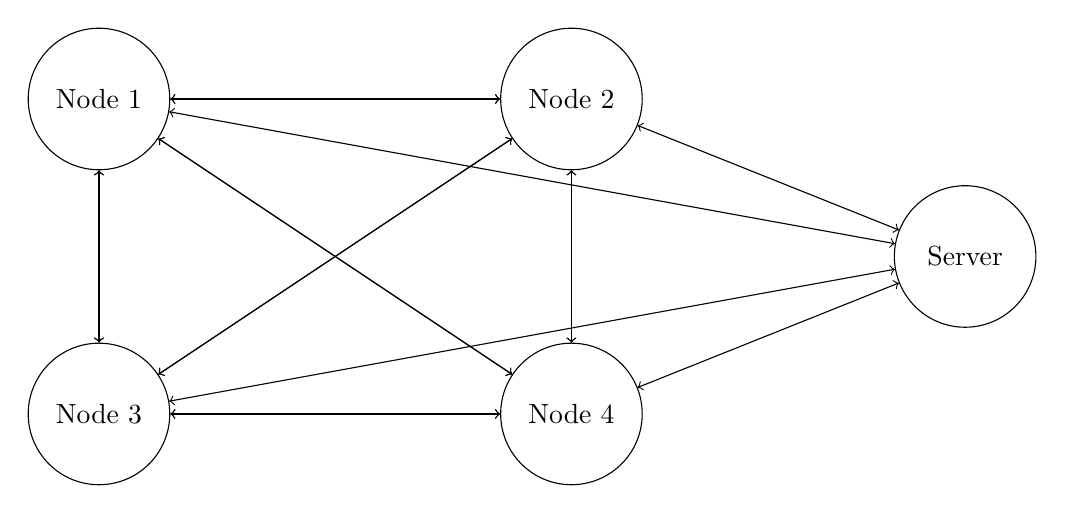
\begin{tikzpicture}
    % Draw central server
    \node[draw, circle, text width=1.5cm, align=center] (server) at (8, 0) {Server};
    
    % Draw nodes
    \node[draw, circle, text width=1.5cm, align=center] (node1) at (-3, 2) {Node 1};
    \node[draw, circle, text width=1.5cm, align=center] (node2) at (3, 2) {Node 2};
    \node[draw, circle, text width=1.5cm, align=center] (node3) at (-3, -2) {Node 3};
    \node[draw, circle, text width=1.5cm, align=center] (node4) at (3, -2) {Node 4};
    
    % Draw communication lines
    \draw[<->] (node1) -- (server);
    \draw[<->] (node2) -- (server);
    \draw[<->] (node3) -- (server);
    \draw[<->] (node4) -- (server);
    
    \draw[<->] (node1) -- (node2);
    \draw[<->] (node1) -- (node3);
    \draw[<->] (node1) -- (node4);
    
    \draw[<->] (node2) -- (node1);
    \draw[<->] (node2) -- (node3);
    \draw[<->] (node2) -- (node4);
    
    \draw[<->] (node3) -- (node1);
    \draw[<->] (node3) -- (node2);
    \draw[<->] (node3) -- (node4);
    
    \draw[<->] (node4) -- (node1);
    \draw[<->] (node4) -- (node2);
    \draw[<->] (node4) -- (node3);
\end{tikzpicture}
\end{center}

% \subsubsection{Central Struct : "Client_data"}
\textbf{1. Central Struct : "Client\_data"}\\
This struct contains all the data that is required for the client to communicate with peers.\\
\begin{verbatim}
    struct Client_data{
        bool received[L];
        string data[L];
        bool complete;
        int port[N];
        const char *ips[N];
        vector<int> broadcast;
        int clientid;
    };
\end{verbatim}
\begin{itemize}
    \item \textbf{received[L]} : This array contains the information about which lines have been received.
    \item \textbf{data[L]} : This array contains the data of the lines that have been received.
    \item \textbf{complete} : This variable tells whether the client has received all the lines or not.
    \item \textbf{port[N]} : This array contains the port numbers of the peers.
    \item \textbf{ips[N]} : This array contains the ip addresses of the peers.
    \item \textbf{broadcast} : This vector contains the information which line is yet to be broadcasted.
    \item \textbf{clientid} : This variable contains the id of the client. 
\end{itemize}

\textbf{2. Driver.cpp}\\
\begin{verbatim}
    int main(){
        // assert((int)client_ips.size() == N);
        vector<pthread_t> clients(N);
        vector<struct Client_data> args;
        vector<int> ports;
        for(int i = 0; i < N;i++){
            struct Client_data temp;
            args.push_back(temp);
            args[i].complete = 0;
            args[i].clientid = i;
            args[i].ips[i] = client_ips[i];
        }
        client((void*) &args[client_id]);
        cout << "Completed Session\n";
        return 0;
    }
\end{verbatim}
This file is driver for starting the cleint. It creates a thread with certain parameters like client id and ip address.\\
\\
\textbf{3. Client.cpp}\\
\textbf{3.1 Client Data Initialization}
\begin{verbatim}
    void* client(void* arg){
        struct Client_data* args = (struct Client_data*) arg;
        pthread_t clientburster, clientrecver, clientcontroller, clientbroadcaster;
        for (int i = 0; i < L; i++) {
            args->received[i] = false;
            args->data[i] = "0";
            // args->broadcasted[i] = false;
        }
        args->complete = 0;
    }
\end{verbatim}
All the cleints will initialize their data and checkpoint array. And they will set the complete variable to 0.\\
\textbf{3.2 Cleint Sub modules}:
\begin{verbatim}
    pthread_create(&clientburster, NULL, clientburst, (void*) &(*args));
    pthread_create(&clientrecver, NULL, clientrecv, (void*) &(*args));
    pthread_create(&clientbroadcaster, NULL, clientbroadcast, (void*) &(*args));
    pthread_create(&clientcontroller, NULL, controller, (void*) &(*args));

    pthread_join(clientburster, NULL);
    pthread_join(clientrecver,NULL);
    pthread_join(clientbroadcaster, NULL);
    pthread_join(clientcontroller, NULL);
\end{verbatim}
This file creates 4 submodules for the client.
\textbf{3.2.1 Clientburst}\\
This thread will continuously receive the packets from the server.\\
\textbf{3.2.2 Clientrecv}\\
This thread will continuously receive the packets from the peer client.\\
\textbf{3.2.3 Clientbroadcast}\\
This thread will continuously broadcast the packets to the peer clients.\\
\textbf{3.2.4 Controller}\\
This thread will continuously check whether the client has received all the packets or not.
\\
\textbf{4. Clientburst.cpp}\\
\textbf{4.1 Creation and Connecting Socket with Server}
\begin{verbatim}
        struct Client_data *needdata = (struct Client_data*) args;
        int status, client_fd;
        struct sockaddr_in serv_addr;
        const char *sendline = "SENDLINE\n";
        char buffer[BUFFER_SIZE];
        if ((client_fd = socket(AF_INET, SOCK_STREAM, 0)) < 0){
            printf("\nSocket creation error \n");
            RETURN(2);
        }
        serv_addr.sin_family = AF_INET;
        serv_addr.sin_port = htons(PORT);
        if (inet_pton(AF_INET, serverIP, &serv_addr.sin_addr) <= 0){
            printf("\nInvalid address/ Address not supported \n");
            RETURN(2);
        }
\end{verbatim}
\textbf{4.2 Sending SENDLINE to Server}
\begin{verbatim}
        while (!needdata->complete) {
            if(send(client_fd, sendline, strlen(sendline), 0) < 0){
                perror("send");
                continue;
            }
\end{verbatim}
\textbf{4.3 Receiving the Data from Server}
\begin{verbatim}
    while(count < 2){
        int x = recv(client_fd, buffer, BUFFER_SIZE, 0);
        if(x < 0){
            perror("recv");
            continue;
        }
        for(int i = 0; i < x; i++){
            if(buffer[i] == '\n') count++;
            mystring += buffer[i];
            if(count == 2) break;
        }
    }
\end{verbatim}
\textbf{4.4 Parsing the Data}
\begin{verbatim}
    while (i < (int)mystring.size() && mystring[i] != '\n'){
        line_num = 10 * line_num + (mystring[i] - '0');
        i++;
    }
    if (line_num >= 0 && line_num < L && !needdata->received[line_num]){
        string data = "";
        for (int j = i + 1; j < (int)mystring.length(); j++){
            data += mystring[j];
            if(mystring[j] == '\n') break;
        }
        cnt++;
        // cout << line_num << endl;
        needdata->data[line_num] = data;
        needdata->received[line_num] = true;
        needdata->broadcast.push_back(line_num);
    }
\end{verbatim}\\

\textbf{5. Clientrecv.cpp}\\
\hspace*{28px}\textbf{Logic : }
\begin{itemize}
    \item Every client will create a socket and bind it to its port. Then it will start receiving for the packets from its peer clients. When it receives the packets, it will parse the data and store it in its data array. It will also update the checkpoint array. The data which would received from the peer client would be in the form of "(line\textbackslash nnumber data)...(line\textbackslash nnumber data)".\\ For every client, we will have N sockets which will try to connect their peer clients. The port number of the socket to which it will try to connect will be the func(client id of peer). We will maintain a vector of sockets which will be used to connect to the peer clients.
    \item As the data received from peer is of the complex form, cleintrecv will try to convert it into the form of "line\textbackslash ndata".
\end{itemize}
\textbf{Converting Data into the required form}
\begin{verbatim}
    reading = "";
    while(count < 2){
        int x = recv(sock, buff, BUFFER_SIZE, 0);
        if(x < 0){
            perror("recv");
            continue;
        }
        for(int i = 0; i < x; i++){
            if(buff[i] == '\n') {
                count++;
            }
            else{
                count = 0;
            }
            reading += buff[i];
            if(count == 2){
                break;
            }
        }
    }
\end{verbatim}
\par We are creating a string reading. We will keep on appending the data to the string reading. When we encounter two consecutive new lines, we will break the loop. It is assumed that the other peers will send the data with appending one extra $\backslash$ n at the end.\\
We know that the underlying protocol TCP is reliable but it uses streams. Hence it could happen that data writtem in kernel socket file is not complete and received in chunks. So to assure that we had recevied all the data, we will keep writing on the client buffer until we encounter two consecutive new lines.\\
Data is parsed in the same way as it was done in clientburst.\\
\\
\textbf{6. Clientbroadcast.cpp}\\
\textbf{Logic : }
\par We have created a queue of lines which are yet to be broadcasted. Whenever we will see that the queue is empty we will record the length of queue at that time. To achieve the functionality of iterating over queue, we have implemented it using a C++ vector. We will iterate over the queue till the length we saw and create a string temp which will contain the data in the form of "line\textbackslash ndata....line\textbackslash ndata". We will then broadcast this data to all the peer clients.\\
\begin{verbatim}
    if(data->broadcast_idx < (int)data->needed_data->broadcast.size()){
        string temp = "";
        int lengthofvector = data->needed_data->broadcast.size();
        while(data->broadcast_idx  < lengthofvector){
            int i = data->needed_data->broadcast[data->broadcast_idx];
            data->broadcast_idx++;
            temp += (to_string(i) + "\n" + data->needed_data->data[i]);
            // upperboundcount++;
        }
        temp += "\n";
        const char *temp1 = temp.c_str();
        if(send(sock, temp1, strlen(temp1), MSG_NOSIGNAL) < 0){
            perror("send");
            continue;
        }
        data->sent = true;
    }
\end{verbatim}

\textbf{7. Calculating the peer ports}
\begin{itemize}
    \item Every client will create N sockets. One socket will always be empty. All the other sockets would be to send the data to other cleints.
    \item The ports of the sockets would be calculated as follows :$$PORTS + (needdata->clientid) * (N) + (i)$$;
    \item Every cleint will connect to the ports : $$(PORTS + (i) * (N) + (need\_data->clientid))$$;
    \item This will ensure that every client will connect to every other client.
\end{itemize}
\begin{figure}[H]
    \centering
    \includegraphics[width=0.8\textwidth]{images/Screenshot from 2023-09-05 11-44-09.png}
    \caption{Client 1 and Client 2 Connections}
    \label{fig:my_label}
\end{figure}

\par The figure show that how Client 1 and Client 2 are connected from all the other peers.\\

\subsection{Fault Recovery and Consistency}
\section{Analysis}
\subsection{N = 1}
\subsection{N = 2}
\subsection{N = 3}
\subsection{N = 4}
\subsection{Relation between Number of Clients and Time}





\end{document}
